% Created 2015-01-13 Tue 11:07
\documentclass[graduation-thesis]{mlarticle}
     \usepackage[dvipdfmx]{graphicx}
\usepackage[utf8]{inputenc}
\usepackage[T1]{fontenc}
\usepackage{fixltx2e}
\usepackage{graphicx}
\usepackage{longtable}
\usepackage{float}
\usepackage{wrapfig}
\usepackage{rotating}
\usepackage[normalem]{ulem}
\usepackage{amsmath}
\usepackage{textcomp}
\usepackage{marvosym}
\usepackage{wasysym}
\usepackage{amssymb}
\usepackage{hyperref}
\tolerance=1000
\usepackage[dvipdfmx]{color}
\usepackage{float}
\usepackage{url}
\author{61106719 情報工学 四年 上司 陽平}
\date{\today}
\title{メモリ共通情報を用いた Live Migration の負荷軽減手法}
\hypersetup{
  pdfkeywords={},
  pdfsubject={},
  pdfcreator={Emacs 24.4.1 (Org mode 8.2.10)}}
\begin{document}

\maketitle

\tableofcontents
\clearpage

\section{はじめに}
\label{sec-1}
\subsection{背景}
\label{sec-1-1}
現在,仮想化技術が様々なサービスを提供するための計算資源管理などの基盤技術として用いられている.
仮想化技術の一つである Live Migration は,クラウドの計算資源管理において有益である.
Live Migration とはある物理マシン上で稼働する仮想マシンを稼働したまま他の物理マシン上に移送する
技術である.
その他にも仮想化技術が利用されている一つの例としてクラウドコンピューティングの PaaS などがあげられる.
クラウドコンピューティングとはネットワークを介して計算資源をユーザに提供するというサービスである.
クラウドコンピューティングの一つとして PaaS というサービスがあり計算資源の管理や利用に効果的である.
PaaS とはアプリケーションを実行するためのプラットフォームをネットワークを介してユーザに提供する
というサービスである.PaaS で提供されるプラットフォームは実際には1つのプラットフォームに1台の
実機があることはなく,仮想化技術により実機マシン1台上に複数の仮装マシンを起動させ,その仮装マシン1台
をプラットフォームとして提供する.よって PaaS では一つの物理マシン上に同じ OS で同様のアプリケーションが
動いている仮想マシンが多く稼働していて,その仮想マシンの1つがプラットフォームとしてユーザに提供される.
(挿図)

上記の例は一部で他にも様々な仮想化技術が存在し,計算資源の管理などの場面で役に立っている.

\subsection{問題点}
\label{sec-1-2}
既存の Live Migration では仮想マシンの全てのメモリを異なる物理マシン上に送信するため
メモリの送信総量が大きい.
Live Migration に必要な時間の大半はメモリ送信であるため,
送信量が大きいと移送に時間がかかる.また送信するページが大きいほど多くのネットワーク資源を使用する.
また,Live Migration は移送時間が長いほど多くの CPU を使用する.
他にも,PaaS のような環境では移送先で移送仮想マシンと同じ内容のメモリを持つ仮想マシンがある場合がある.
その場合,移送する仮想マシンの移送先に同じ内容のあるメモリページは再利用可能なので,
そのメモリページは移送せず移送先で共有し再利用することが可能である.(挿図)

\subsection{提案}
\label{sec-1-3}
PaaS 環境における Live Migration で移送仮想マシンのメモリと同様のメモリが移送先物理マシンに
あるときはそのメモリは移送せず,移送先で共有し再利用する.
移送メモリの総量を減らす.それによって移送時間を短くし,使用ネットワーク量も減らす.
移送時間を短くすることで CPU の使用率も削減する.

\subsection{実験}
\label{sec-1-4}
既存の Live Migration より提案手法の Live Migration の方が移送時間も短く
ネットワークと CPU の使用量が少ないことを示した.

\clearpage
\section{仮想化技術}
\label{sec-2}
現在仮想化技術は様々なサービス提供の基盤技術として使用されている.
本章では仮想化技術の全般の話からクラウドコンピューティングにおける仮想化,Live Migration 
についてなど詳細な内容を説明する.
\subsection{仮想化}
\label{sec-2-1}
\subsubsection{仮想化とは}
\label{sec-2-1-1}
現在 IT の複雑さが増しており,取り扱いも比例して複雑化している.そのような技術を簡単で扱いやすい
ものにするのが仮想化の根本的な考え方である.つまり IT における仮想化とは
「ストレージ,メモリなどの計算資源の複雑な技術特性を隠蔽し,論理的な利用単位にし提供する技術」
と考えることができる.その利用単位の粒度によって仮想化は様々な種類にわけられる.
粒度の小さい例で言えばマルチプロセッサがあげられる.これは CPU を仮想化する技術で,
物理的には一つしかない CPU を時間単位などで使用を分配することであたかも複数の CPU が
動作しているように振舞わせる技術である.また物理リソースの特性を隠蔽し,ユーザにサービスを提供する
OS も仮想化といえる.大きな粒度で見ればサーバのクラスタリング技術などがあげられる.
クラスタリング技術とは複数のコンピュータを繋げて,クライアントには1台のコンピュータだけが動作している
かのように振る舞わせる技術である.
\subsubsection{サーバ仮想化}
\label{sec-2-1-2}
このように IT システムでは色々な仮想化技術で使用されている.そのような技術のひとつとして
サーバの仮想化という技術がある.これは物理サーバを論理的な構成単位に分割して利用する技術である.
本来 OS は,CPU,メモリなどの物理資源を全て使用しているように振る舞う.そのため通常は,
複数の OS で一つの物理資源を使用することはできない.サーバ仮想化技術では
実際の物理マシンの上で仮想マシンを作り出し,OS にはその仮想マシンを与えることで
あたかも実際に物理マシンを与えられている様に振る舞わせることができる.(挿図)

サーバの仮想化の利点は多々ある.その利点について説明する.
\begin{itemize}
\item リソースの効率的な利用\\
     サーバ仮想化を行っていないと
マシン上では一つの OS しか動かないため,一つの OS が全ての物理資源を使用して
その OS が使用しない物理資源が存在する.一方,仮想化を行うことで物理資源を複数の OS で効率的に分配し
有効に利用することができる.
\item システムの柔軟性\\
     サーバを物理的な制約を考えることなく管理できる.サーバに与えられているのは仮想マシンで,
多くの仮想マシンがが一台のマシンで稼働するので多大数を一気に管理することができる.
またハードウェアのデバイスチェックなどの時間も省略できるので立ち上げの高速化や
Live Migration により仮想マシンを稼働させたまま他の物理マシンに移送することで
物理マシンのメンテナンスも容易になる.
\item 省コスト・省電力\\
     物理サーバの運用台数を削減できるので電力の消費,設置スペースの削減が行える
\item 障害性\\
     仮想マシンごとは完全に分離されているのでいずれかの仮想マシン上の OS がクラッシュしても
他のマシンには影響をあたえない.
\end{itemize}
このようにサーバ仮想化には様々な利点がある.
\subsubsection{サーバ仮想化方式}
\label{sec-2-1-3}
サーバの仮想化には様々な方法が存在する.
その方法は大きく二つに分類され,ホスト OS 型とハイパーバイザ型に大別される.
\begin{enumerate}
\item ホスト OS 型
\label{sec-2-1-3-1}
図(挿図)のように物理マシン上でひとつのホストとなる OS が稼働し,その OS 上で
仮想マシン・モニタを起動する方式.仮想マシン・モニタとは仮想マシンを OS に提供する
ソフトウェアの事を指す.ホスト OS 型は既存のマシン環境で,
他のアプリケーションを使用するようにインストールし,起動することが
できるので仮想化のために新たに環境を用意する必要がない.一例として Macintosh マシン上で
アプリケーションの VirtualBox\cite{virtualbox} などの仮想マシン・モニタを
用いて Windows を起動するなどということができる.
一方,仮想マシン・モニタに与えられる CPU 処理時間がホストマシンの OS の
アプリケーションのスケジューリング依存になるので,ホスト OS で多くのアプリケーションを
起動している場合や多数のゲスト OS を起動している場合性能があまり出ないことがある.
\item ハイパーバイザ型
\label{sec-2-1-3-2}
ホスト OS 型だと仮想マシンと物理マシンの間にはホスト OS と仮想マシン・モニタの二層が存在する.
一方ハイパーバイザ型では図(挿図)のように物理マシンと仮想マシンの間にはハイパーバイザと呼ばれる
仮想マシン・マシンモニタのみが存在する.ハイパーバイザによってハードウェアは仮想化され
OS に提供される.ホスト OS が存在せずハイパーバイザが直に物理資源を利用するため
ハイパーバイザがゲスト OS へ与えられる CPU のスケジューリング行うことができる.
そうすることによりホスト OS 型と比べると,効率的にかつ安定的に CPU をゲスト OS に
割り当てることができる.vmware の vSphere\cite{vsphere},citrix の XenServer\cite{xenserver},
Microsoft の Hyper-V\cite{hyper-v}など
商用の仮想化ソフトウェアとしてハイパーバイザ型の商品も多数存在する.
オープンソースでの開発も行われていて,XenSever の元である Xen\cite{xen} や Linux カーネルに
マージされている KVM\cite{kvm} などがあげられる.
\begin{itemize}
\item 完全仮想化
ページ数稼ぎたい場合は完全仮想化の話とかする
\end{itemize}
\end{enumerate}
\subsection{クラウドコンピューティングにおける仮想化技術の利用}
\label{sec-2-2}
\subsubsection{クラウドコンピューティングとは}
\label{sec-2-2-1}
クラウドコンピューティングとは,インターネットを介して,必要に応じた計算資源を
ユーザに提供するサービスである.ユーザは実際の物理マシンを意識せず計算資源を利用する
ことができる.

従来ユーザがシステムを構築しようとしたとき,物理マシンを用意し,
そのうえに基幹ソフトウェアをインストールし,必要な環境を用意することで
初めて利用を開始していた.また使用を開始した後も
物理マシンのメンテナンスから,ソフトウェアの環境の管理など様々な管理コストが掛かっていた.
一方クラウドコンピューティングでは必要な環境をユーザ登録などを済ませることで
すぐさま利用することができる.また利用するユーザは物理マシンのメンテナンスなどをサービス提供者に
任せることができる.
クラウドコンピューティングでは,下位層から上位層様々な層のサービスを提供する.
具体的には下位層では基幹ソフトウェアも何も用意していないようなマシンから
上位層であればソフトウェアのみのサービスなどである.
ユーザは自分の提供された計算資源より上位層の部分だけ管理すればよいので従来必要だった
管理コストを他に割り当てることができる.
例えばストレージのみをクラウドコンピューティングで利用する場合,
保存したファイルのバックアップ作業はサービス提供元が行ってくれるので
バックアップの為に RAID を構成するなどの管理作業からユーザは解放されることになる.

\subsubsection{PaaS とは}
\label{sec-2-2-2}
クラウドコンピューティングの一つのサービス体系で,アプリケーションが稼働するための
ハードウェアや OS などのプラットフォーム一式をインターネットを介して提供する
サービスである.

プラットフォームを提供されるユーザは開発,運用のためのハードウェアや OS ,開発環境,
ミドルウェアなどのプラットフォーム一式を自ら構築しなくてよい.
ハードウェアのメンテナンスや障害対応もしなくてよくなる.
またユーザは利用規模に応じたサービスを受けることができるので利用規模に応じた柔軟な計算資源の
利用をすることができる.

PaaS 提供者は,プラットフォーム一式を大規模なデータセンタなどに用意して,
顧客企業へネットワークを通じてプラットフォーム一式を提供する.
データセンタ内では複数の物理マシンサーバが用意され,プラットフォームの管理には
仮想化技術が利用されている.
各物理マシン上で仮想化技術により複数の仮想マシンが稼働しており,その仮想マシン上に同様の構成の
プラットフォーム一式が構築される.(挿図)ユーザにはその仮想マシン上のプラットフォーム一式が提供される.
PaaS 提供者は各物理マシンの整備からミドルウェア,開発環境などの管理をすることになる.

具体的な一例として Microsoft の Azure\cite{azure} をあげてみる.
Azure のサービスは IaaS,PaaS,ストレージなど多岐にわたる.
そのうち, PaaS のサービスでは Azure Websites というサービスがある.
これは管理されたプラットフォームをユーザに提供し,ユーザはプラットフォーム上で
Python,Java,PHP,ASP.NET など様々な言語を使用しランタイムの Web アプリケーション
を使用することができる.
プラットフォームは Windows Serever に手を加えたものが使われており,
ミドルウェアなども含め多くの同じプログラムを起動している仮想マシンが複数個
データセンタの物理マシン上に存在している.

\subsubsection{IaaS と SaaS説明}
\label{sec-2-2-3}
ページ数足りなかったら
\subsection{Live Migration}
\label{sec-2-3}
\subsubsection{Live Migration とは}
\label{sec-2-3-1}
Live Migration とは,アプリケーションを稼働したまま仮想マシンを他の物理マシンに移送する
技術である.Live Migration の機能は様々な仮想化ソフトに実装されている.
ホスト OS 型である,Virtualbox\cite{virtualbox}では「テレポート」という機能として,
ハイパーバイザ型では VMware の vSphere\cite{vsphere} では「VMotion」,
Citrix XenServer\cite{xenserver} では「XenMotion」,
Microsoft の Hyper-V\cite{hyper-v} やオープンソースの KVM\cite{kvm}.
Xen\cite{xen}ではそのまま「Live Migration」という名前の機能として使われている.

\subsubsection{Live Migration の使用}
\label{sec-2-3-2}
Live Migration が使用される場面を説明する.
まず複数の仮想マシンの負荷総量が物理マシンの処理能力を上回った
場合の利用についてあげる.
元来,仮想化を導入する理由の一つにハードウェアの効率的利用があげられる.
高性能のハードウェアの計算資源を常に全て利用することは難しいので,
複数のサーバをその一台に集約することで計算資源を効率的に利用することができる.
しかしそのような使い方をすると一台の物理マシン上で稼働する各仮想マシンが
高負荷な処理を行ったとき,物理マシンの処理能力を複数の仮想マシンの負荷が上回って
しまうことがある.上回った場合,各仮想マシンへの CPU 割当は満足のいくものではなくなり
各仮想マシン上で動いているサービスの性能が低下してしまう.
このような場合に Live Migration の使用が考えられる.
負荷総量の上昇を検知できた段階で一部の仮想マシンを他の物理マシンに移送すれば
負荷総量が物理マシンの処理能力を超さないで済む.(図\ref{high_load})
引用OKか確認?どちらにしろ図が悪い?
\begin{figure}[H]\begin{center}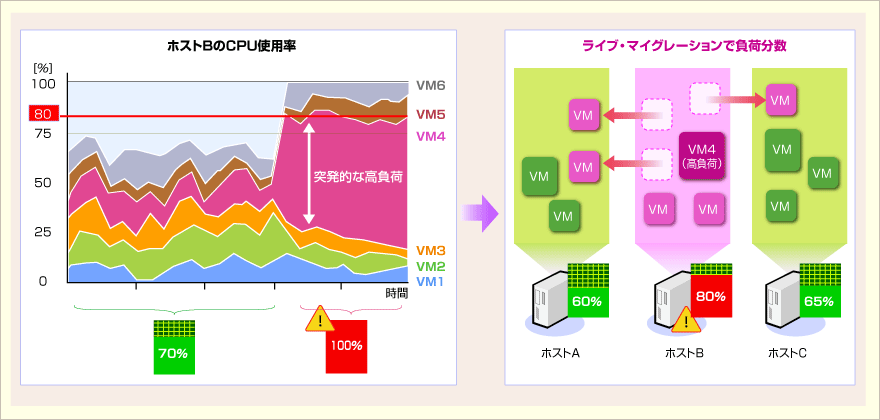
\includegraphics[width=16.0cm]{./img/high_load.png}\caption\{ 高負荷分散 (引用:\cite{livemigration})\}\label{high_load}\end{center}\end{figure}
次にあげられるのが物理マシンのメンテナンスをする場合である.
ホストマシン上で稼働する仮想マシン・モニタはバグ修正,機能向上のために
定期的にパッチがリリースされる.そのため定期的にホストマシンを停止し,
仮想マシン・モニタを更新する.その他にもメモリの故障による
ハードウェアの交換時などにもホストマシンを一旦停止することになる.
ホストマシンを停止する場合,ホストマシン上の仮想マシンもシャットダウンされてしまう.
しかし仮想マシンでサービスを動かし続けている場合は,サービスを中断するわけにはいかない.
このような場合仮想マシンのサービスを停止することなく他のホストマシンに移送する
Live Migration が用いられる.
Live Migration によってメンテナンスをしたいホストマシン上の全ての仮想マシンを
他のホストマシン上に待避させることができる.全ての仮想マシン待避後,
ホストマシンを停止しハードウェアのメンテナンスを行ったり,再起動を伴う
更新などを行うことができる.(図\ref{maintenance})
\begin{figure}[H]\begin{center}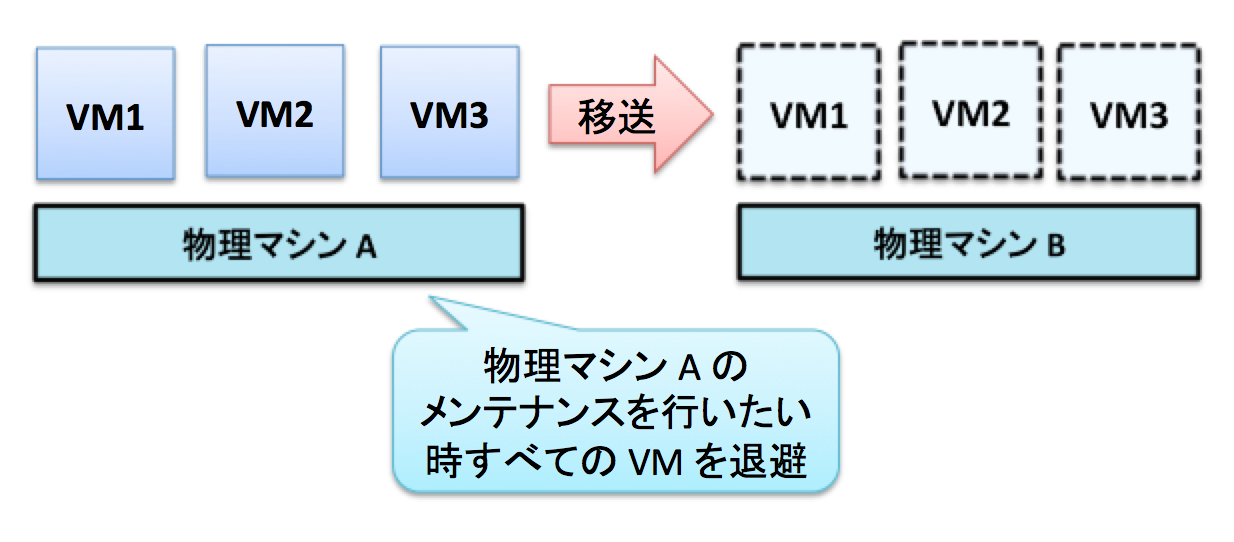
\includegraphics[width=16.0cm]{./img/maintenance.png}\caption\{ メンテナンス時 (引用:\cite{livemigration})\}\label{maintenance}\end{center}\end{figure}
\subsubsection{移送する対象と方法}
\label{sec-2-3-3}
Live Migration を行うにあたっての移送する対象と
その移送方法について説明する.
まず仮想マシンを移送するということは,大きく二つにわけて,
仮想マシンのディスクとメモリを移送するということになる.
この仮想マシンのディスクとメモリの移送方法は二つにわかれる.
一つはディスクとメモリ両方を移送先に移送する方法で,
もう一つは移送先とディスクを共有しておきメモリだけ移送する方法である.
\begin{itemize}
\item 両方とも移送先に移送する\\
      まず一つ目の移送方法は,仮想マシンのメモリもディスクも
どちらも移送する方法である.マシンの配置例は図\ref{arrangement1}
のようになる.ここではメモリとディスクと両方を Live Migration する機能をもつ
vSphere を例に説明する.
この場合 vSphere の移送元ホストマシンは移送先と移送元ホストマシン同士の
vMotion (Live Migration) 用の回線を使い
まずストレージを移送先ホストマシンに移送する.
その後メモリを移送先に移送することで移送が完了する.
詳しい移送の仕組みについては後述する.
ディスクを共有する方法では共有ディスクを用意しなくてはいけないが
両方送れることで用意なしで Live Migration が可能になる.
しかし,ディスク送信をするため大きい容量を移送しなければならないのでネットワークを圧迫したり,
移送時間が長い.
他にも citrix の XenServer の Storage XenMotion や 
Microsoft の Hyper-V の Shared Nothing Live Migration などがある.
\cite{xenserver_migration}
\begin{figure}[H]\begin{center}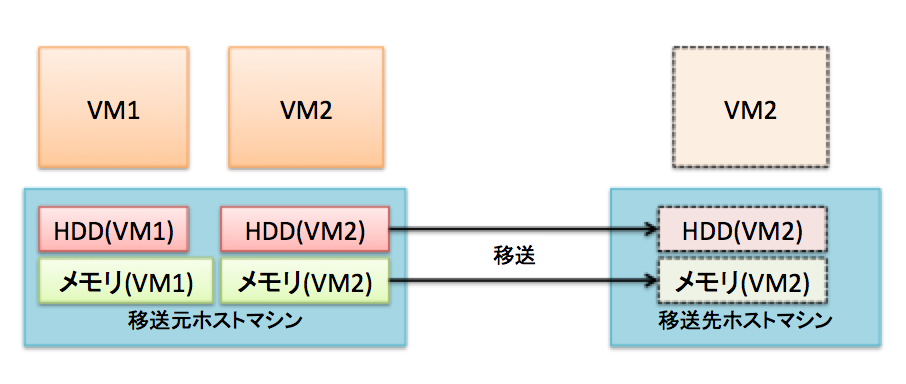
\includegraphics[width=16.0cm]{./img/arrangement1.png}\caption\{ マシン配置例1 (引用:\cite{vmotion})\}\label{arrangement1}\end{center}\end{figure}
\item ディスクを共有しメモリのみを移送する\\
      もう一つの方法は図\ref{livemigration}の様にストレージを共有し,
メモリのみを移送先に移送する方法である.
移送の流れとしては(1)メモリを移送先に移送し,(2)移送先の仮想マシンを稼働させ,
ストレージは共有ストレージを使用するようにするという流れになる.
この方法では共有ストレージを用意しなくてはならないが移送するのは
メモリだけなのでディスクとメモリ両方を移送する方法よりも大きく移送時間を減らすことができる.
共有の方法には NAS(Network-attached storage)などがあげられる.
本提案での Live Migration はこの方法をとる.
\begin{figure}[H]\begin{center}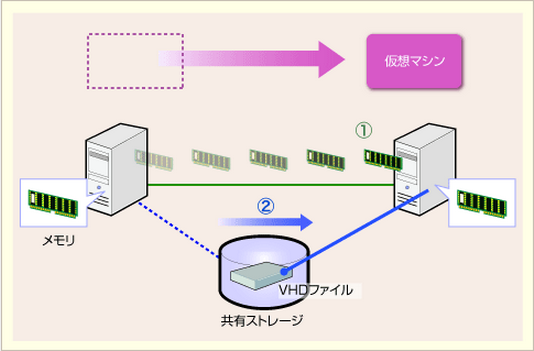
\includegraphics[width=16.0cm]{./img/arrangement2.png}\caption{ マシン配置例2この図は書き換える}\label{arrangement2}\end{center}\end{figure}
\end{itemize}
\subsubsection{移送の仕組み}
\label{sec-2-3-4}
\begin{itemize}
\item ストレージの移送\\
      本提案ではディスクを共有した,メモリのみの移送をする Live Migration を使用するので,
ストレージの移送方法については vSphere の移送方法のみを参考として説明する.
vSphere のディスク移送には並列して二つのプロセスが稼働する.(図\ref{vmotion})
一つはストレージ全体を線形的に移送先にコピーする Bulk Copy プロセスと,
もう一つは IO をミラーリングするプロセスである.
IO ミラーリングのプロセスは OS の IO 操作を監視して,IO 操作を移送元ホストの
現在使用中のストレージと移送先ホストのコピー中のストレージに反映させる.
ふたつのプロセスはトランスポートのバッファリングを用いて非同期的に移送先に送信される.
何故バッファリングを行い非同期的に行うかというと,
同期的に行うと,ネットワークのレイテンシによっては IO がとても混雑してしまい,
VM の性能を下げてしまうことがあるからである.
Bulk Copy プロセスが全てのストレージを移送先にコピーすると,Bulk Copy プロセスは
終了し,IO ミラーリングプロセスのみが稼働し続けた状態でメモリの移送を開始する.
\begin{figure}[H]\begin{center}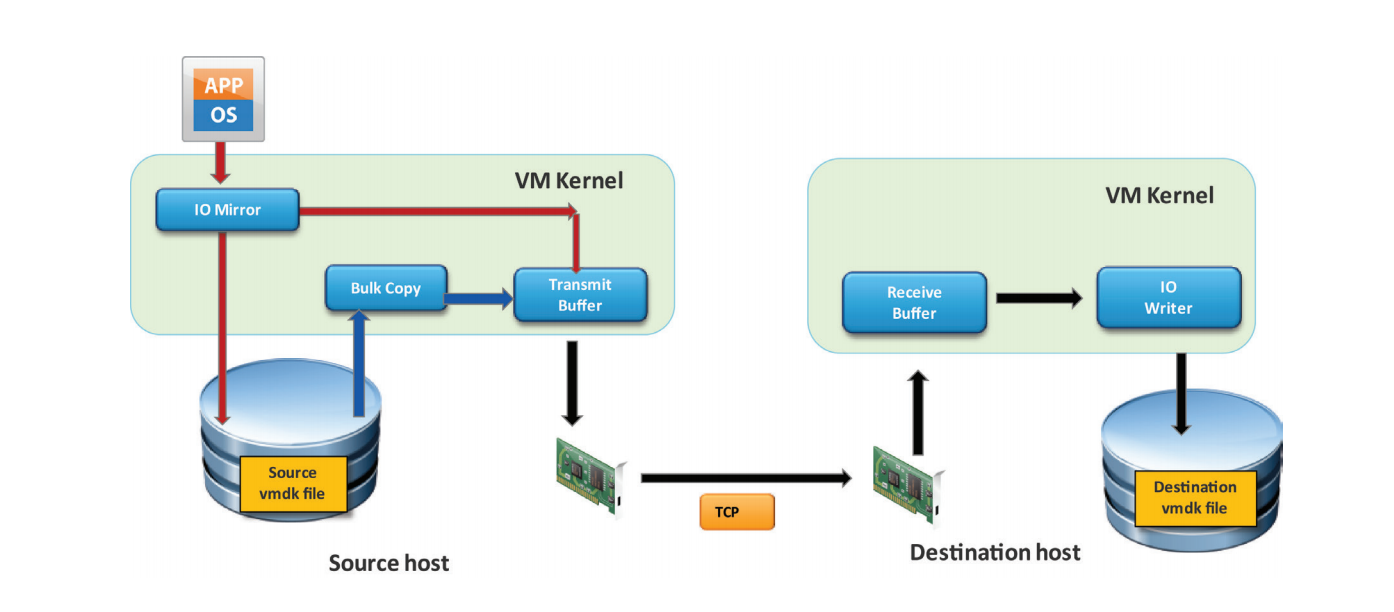
\includegraphics[width=16.0cm]{./img/vmotion.png}\caption{ ストレージ vMotion}\label{vmotion}\end{center}\end{figure}

\item メモリの移送\\
      メモリの移送は主に pre-copy が使用されている.\cite{precopy}
vSphere\cite{vsphere} の vMotion(vSphere 特有の Live Migration の機能の名前)\cite{vmotion} 
や Hyper-V\cite{hyper-v} の Live Migration \cite{hyper-v_live},
オープンソースの Xen などで実際に pre-copy が使用されている.
ここでは pre-copy について説明する.
pre-copy では六つのステージによって Live Migration を行う.
動作の流れを図\ref{pre-copy}に示す.ステージ0では 移送したい VM を稼働
することができる程の計算資源を持った移送先ホストマシンを選択する.
ステージ1では移送先ホストに移送を開始することを通知する.また送信ができる程の計算資源が
あるかどうか確認する.ステージ2ではメモリを繰り返し送信する.このステージでは
まず全てのページを送信する.送信中には dirty にされるページ(稼働中の仮想マシンが更新したページ)を
記録しておく.後続のイテレートでは dirty にされたページを再送する.
ページの再送時にも dirty にされたページを記録し,後続のイテレートとそのページを再送する.
この移送中に更新されたメモリを再送するという動作を,管理者が定めた一定の閾値に達するまで繰り返す.
閾値にはメモリの再送フェーズを行う回数の最大値や,再送するページの数の最小値などが用いられる.
ステージ3では仮想マシンをサスペンドし,残りの dirty になったページや CPU レジスタや
プログラムカウンタなどを移送する.
この移送が終わった状態では,移送元ホストマシンと移送先ホストマシンに同様の仮想マシン
イメージがある状態になる.
ステージ5では移送先ホストが移送元ホストに移送が終了したことを通知する.
この通知により移送元ホストは整合性のとれたメモリの移送を完了したとして,移送元の
仮想マシンを廃棄する.よって仮想マシンのイメージは移送先のもののみになる.
ステージ6では移送した仮想マシンを再開する.
この時デバイスドライバの設定や,仮想マシンの IP アドレスの設定などを行う.
\begin{figure}[H]\begin{center}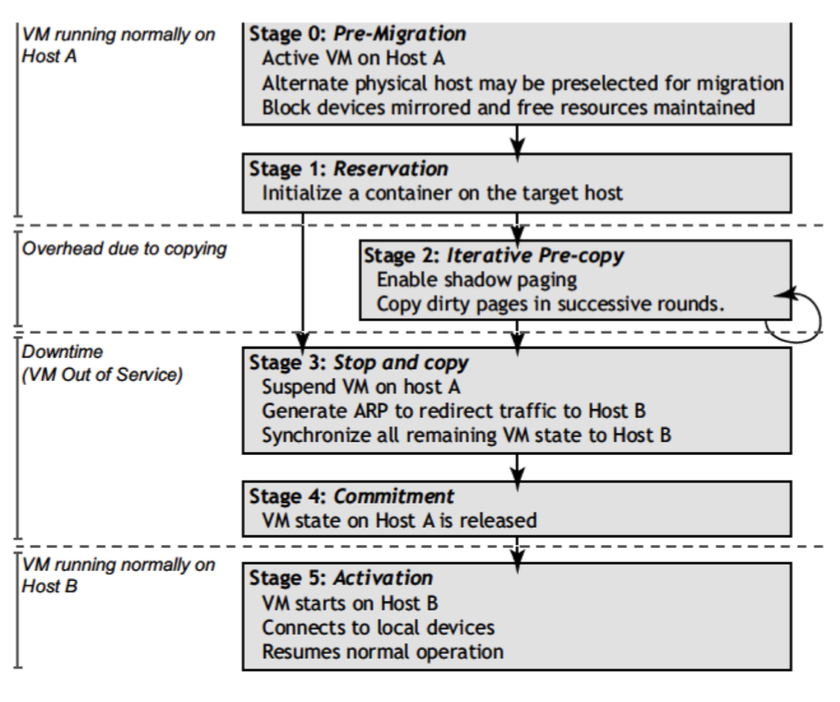
\includegraphics[width=16.0cm]{./img/pre-copy.png}\caption{ pre-copy の流れ}\label{pre-copy}\end{center}\end{figure}
\end{itemize}
\subsection{仮想マシン間のページ共有技術}
\label{sec-2-4}
仮想化技術により一つの物理マシンに複数台の仮想マシンが存在する場合,
各々の仮想マシンが同じ内容のメモリページを重複して持つ場合がある.
そのようなページを仮想マシン間で共有する方法を説明する.
\subsubsection{Transparent Page Sharing}
\label{sec-2-4-1}
仮想マシン間で重複した内容のメモリページを共有する技術は
Disco\cite{disco}で 
{\it transparent page sharing}
として導入された.
同じ OS が起動していた場合,テキストデータ領域などが
共有できる場合がある.他にも同じアプリケーションを動かしているとき
そのアプリケーションのテキストデータ領域や,場合によっては使用する
データも共有できる場合がある.
そのような場合重複したメモリページに対して一つの物理ページを用意してやり,
どのメモリページもその一つの物理ページを参照する様にすればメモリの使用量を
減らすことができる.
重複排除したメモリページは read-only に設定しておき,
書き込みを行った時に page fault が起こるようにしておく.
page fault が起きた場合,新しくページを作った上で変更した内容のページを作成する.
この機能は仮想マシン・モニタに実装されており
ゲストマシン OS にとっては名前の通り透過的なメモリシェアとなっている.

\subsubsection{メモリ共有}
\label{sec-2-4-2}
ここではメモリを効率的に共有する方法\cite{sharing}を説明する.
メモリを共有するとき毎回 4kbyte のページ内容を全て比較していると計算量はかなり
多くなってしまう.また単にページ同士を総当たりで比べるとなるとページ数の自乗回の
比較が必要になってしまう.
そこで効率的な比較をする方法として
メモリ内容から計算されるハッシュ値によるハッシュテーブルの使用があげられる.
(図\ref{hashtable})
具体的には,メモリの比較時にメモリの内容からハッシュ値を計算してハッシュテーブルから
同じハッシュ値をもつページを引く.もし同じハッシュ値を持つページが存在すれば
ページの内容を比較して,同じならば TPS (Transparent Page Sharing) で共有する.
もし同様のハッシュ値がなかった場合はハッシュテーブルに登録だけして終わる.
このようにすることでページの内容が違う場合はハッシュ値の比較だけで済むため
比較の計算量が減る.またページの比較回数もページの自乗回かかっていたものが
ハッシュテーブルを利用して同じハッシュ値のみを検索し比較することで検索回数は大幅に減らすことができる.
検索が O(1) の理想的なハッシュテーブルを作成した場合は検索回数はページ数回で済むことになる.
しかし,仮想マシン・モニタがラージページに対応しているとページサイズは 4kB から
2 MB と 512 倍に跳ね上がるためページ共有の機会がとても少なくなる.
その場合共有をあまりしないのにハッシュ値を計算するために CPU を使用することになる.
Microsoft は仮想マシンのページ共有は将来的に必要のないものになると考え
Hyper-V にはメモリ共有機能は実装されていない.
現在メモリ共有は ESX を内包する vSphere の TPS,オープンソースの KVM では
ivshmem(Inter-VM shared memory) という機能名で実装されている.

\begin{figure}[H]\begin{center}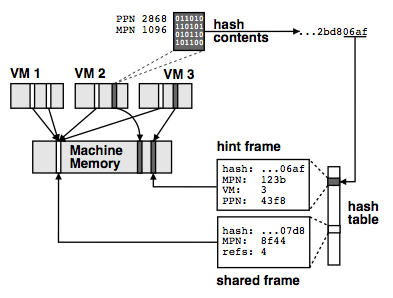
\includegraphics[width=16.0cm]{./img/hashtable.png}\caption{ ハッシュテーブルによるメモリ比較)}\label{hashtable}\end{center}\end{figure}

\clearpage
\section{関連研究}
\label{sec-3}
\subsection{MiyakoDori}
\label{sec-3-1}
ここはポストコピーにするか
[Akiyama et al. IEEE Cloud’ 12]
\subsection{Towards Unobtrusive VM Live Migration for Cloud Computing Platforms}
\label{sec-3-2}
ここは古藤さんの論文みせてもらおう
[Koto et al.  APSYS’ 12]
\subsection{まとめ}
\label{sec-3-3}
移送時のメモリ削減手法は色々あるが PaaS 環境における再利用可能なページを転送をしない手法がない.
他の手法と比べ自分のを使うとどのようになるかの事実を述べる

\clearpage
\section{提案手法}
\label{sec-4}
\subsection{概要}
\label{sec-4-1}
PaaS 環境においては dst 側に転送したいページと同じページが存在する可能性が高い.(この言い方は主観的)
同じ設定の VM を src と dst で稼働させているような 
PaaS 環境において,ページ転送を削減する.といった感じで書く.
移送時間が減ると dirty が減って嬉しいってことあたりはここにかく
\subsection{効率的な非移送ページの探索}
\label{sec-4-2}
VM 間での共有は常にハイパーバイザーで行われている(ということにして).
PaaS 環境では移送元で共有できているページは移送先にもある可能性が高いため
既に共有済みのページは移送先でも共有できる可能性が高いこと述べる.\\
   共有ページだけみれば本提案で削減したいページについてはとても効率的に見つけれることができることを述べる.
本当はハッシュコリジョンについての論文のリファーなどもここでしたい

\clearpage
\section{実装}
\label{sec-5}
がっつり書く
\subsection{全体像}
\label{sec-5-1}
xen を用いることを述べる.\\
   非転送メモリの決定フェーズを既存のライブマイグレーションの途中に設けて,
それ以降は既存のマイグレーションを(pre-copy)を行う.\\
   モジュールの全体像も書く
\subsection{(メモリ共有モジュール)}
\label{sec-5-2}
今回の実装についてはメモリ共有モジュールでのメモリ管理などが結構な量を占めているので,
実装でページ数を稼ぐならメモリ共有モジュールも自分で作ってこれが大変だったなど書けるのですが,
本提案についてメモリ共有モジュールは本質的な実装ではないので書かないほうが良いでしょうか?
\subsection{非転送メモリの確認方法}
\label{sec-5-3}
非転送ページ候補として共有時に作られたハッシュ値を用いて移送先に同じページがあるかどうかを確認する.
そのために作ったハイパーコールとかも少し紹介する(?)
\subsection{非転送ページの共有}
\label{sec-5-4}
非転送ページを確定したのち,移送先でページを共有することによって,ページの転送量を減らす
\subsection{Live Migration への組み込み}
\label{sec-5-5}
既存の実装の dirty の管理方法,移送先でのアロックしたページの管理方法を説明して,
本提案実装が辻褄の合う様に組み込めていることを説明する

\subsection{実験のスクリプト関連の苦悩とかも書いていいのかな笑}
\label{sec-5-6}
\clearpage
\section{実験}
\label{sec-6}
\subsection{非転送ページの量を調整した本実装の実験}
\label{sec-6-1}
\subsubsection{目的}
\label{sec-6-1-1}
本提案で CPU やネットワークの消費を抑えることを示す.
移送時間が減ることも示す
\subsubsection{実験方法}
\label{sec-6-1-2}
PaaS 環境を想定して,各VM に同じページをもたせて本提案の実験をした.\\
    同じページの量は調整できる.
\subsubsection{実験結果}
\label{sec-6-1-3}
費転送ページが多い程移送時間が短くなり CPU やネットワークの使用時間も削減できているので
浪費を抑えることができた.\\
    (移送時間が短くなったのでその分 CPU やネットワークの浪費は抑えられたという結果の持っていきかたは
強引すぎるでしょうか.)
\clearpage
\section{おわりに}
\label{sec-7}
\subsection{conclusion}
\label{sec-7-1}
\subsection{今後の課題}
\label{sec-7-2}
\begin{itemize}
\item 実際の PaaS 環境を想定した memcached などを用いた実験をする
\item VM のメモリ量を増やしても同様に動作するかなどの検証
\end{itemize}
\clearpage
\section{謝辞}
\label{sec-8}
\section{参考文献}
\label{sec-9}
\begin{thebibliography}{99}
\bibitem{virtualbox} VirtualBox 
\url{https://www.virtualbox.org/}
\bibitem{virtual_beginner} 仮想化入門\ 
\url{http://www.plathome.co.jp/solution/virtualserver/introduction/}
\bibitem{virtual_taizen} 浅見直樹 日経BP社 
「仮想化大全」 p14-17
\bibitem{vsphere} vSphere
\url{http://www.vmware.com/jp/products/vsphere}
\bibitem{xenserver} XenServer
\url{http://www.citrix.co.jp/products/xenserver/xenserver.html}
\bibitem{hyper-v} Hyper-V
\url{http://www.microsoft.com/ja-jp/server-cloud/windows-server/hyper-v.aspx}
\bibitem{xen} Xen
\url{http://xenproject.org/}
\bibitem{kvm} KVM
\url{http://www.linux-kvm.org/page/Main_Page}
\bibitem{cloud_computing} IT 用語辞典\ 
\url{http://e-words.jp/}
\bibitem{azure} Azure\ 
\url{http://azure.microsoft.com/ja-jp/}
\bibitem{vmotion} Vmware vSPhere 5.1 vMotion
Architecture, Performance, and Best Practices
\bibitem{hyper-v_live} Hyper-V のライブマイグレーションの説明\\
\url{http://technet.microsoft.com/ja-jp/library/hh831435.aspx}
\bibitem{livemigration} Hyper-V 2.0 のライブ・ライブマイグレーションの基礎知識\\
\url{http://www.atmarkit.co.jp/ait/articles/0912/16/news102.html}
\bibitem{xenserver_migration} Storage XenMotion: 
Live Storage Migration with Citrix XenServer
\bibitem{precopy} Christopher Clark, Keir Fraser, Steven Hand, Jacob gorm Hansen,
Eric Jul, Christian Limpach, Ian Pratt and Andrew Warfield. Live migration of virtual machines,
NSDI'05 Proceedings of the 2nd conference on Symposium on Networked Systems Design \& 
Implementation - Volume 2, Pages 273-286 , 2005.
\bibitem{sharing} Carl A. Waldspurger. Memory Resource Management in VMware ESX Server,
Fifth Symposium on Operating Systems Design and Implementation (OSDI ’02), 
Pages 181-194, Dec. 2002.
\bibitem{disco} Edouard Bugnion, Scott Devine, Kinshuk Govil, and Mendel Rosenblum. 
“Disco: Running Commodity Oper- ating Systems on Scalable Multiprocessors,
” ACM Trans- actions on Computer Systems, 15(4), November 1997.
\end{thebibliography}



とりあえず見つけた論文少し目を通そうか
% Emacs 24.4.1 (Org mode 8.2.10)
\end{document}
